\section{Packet transactions}
%\begin{figure}
%  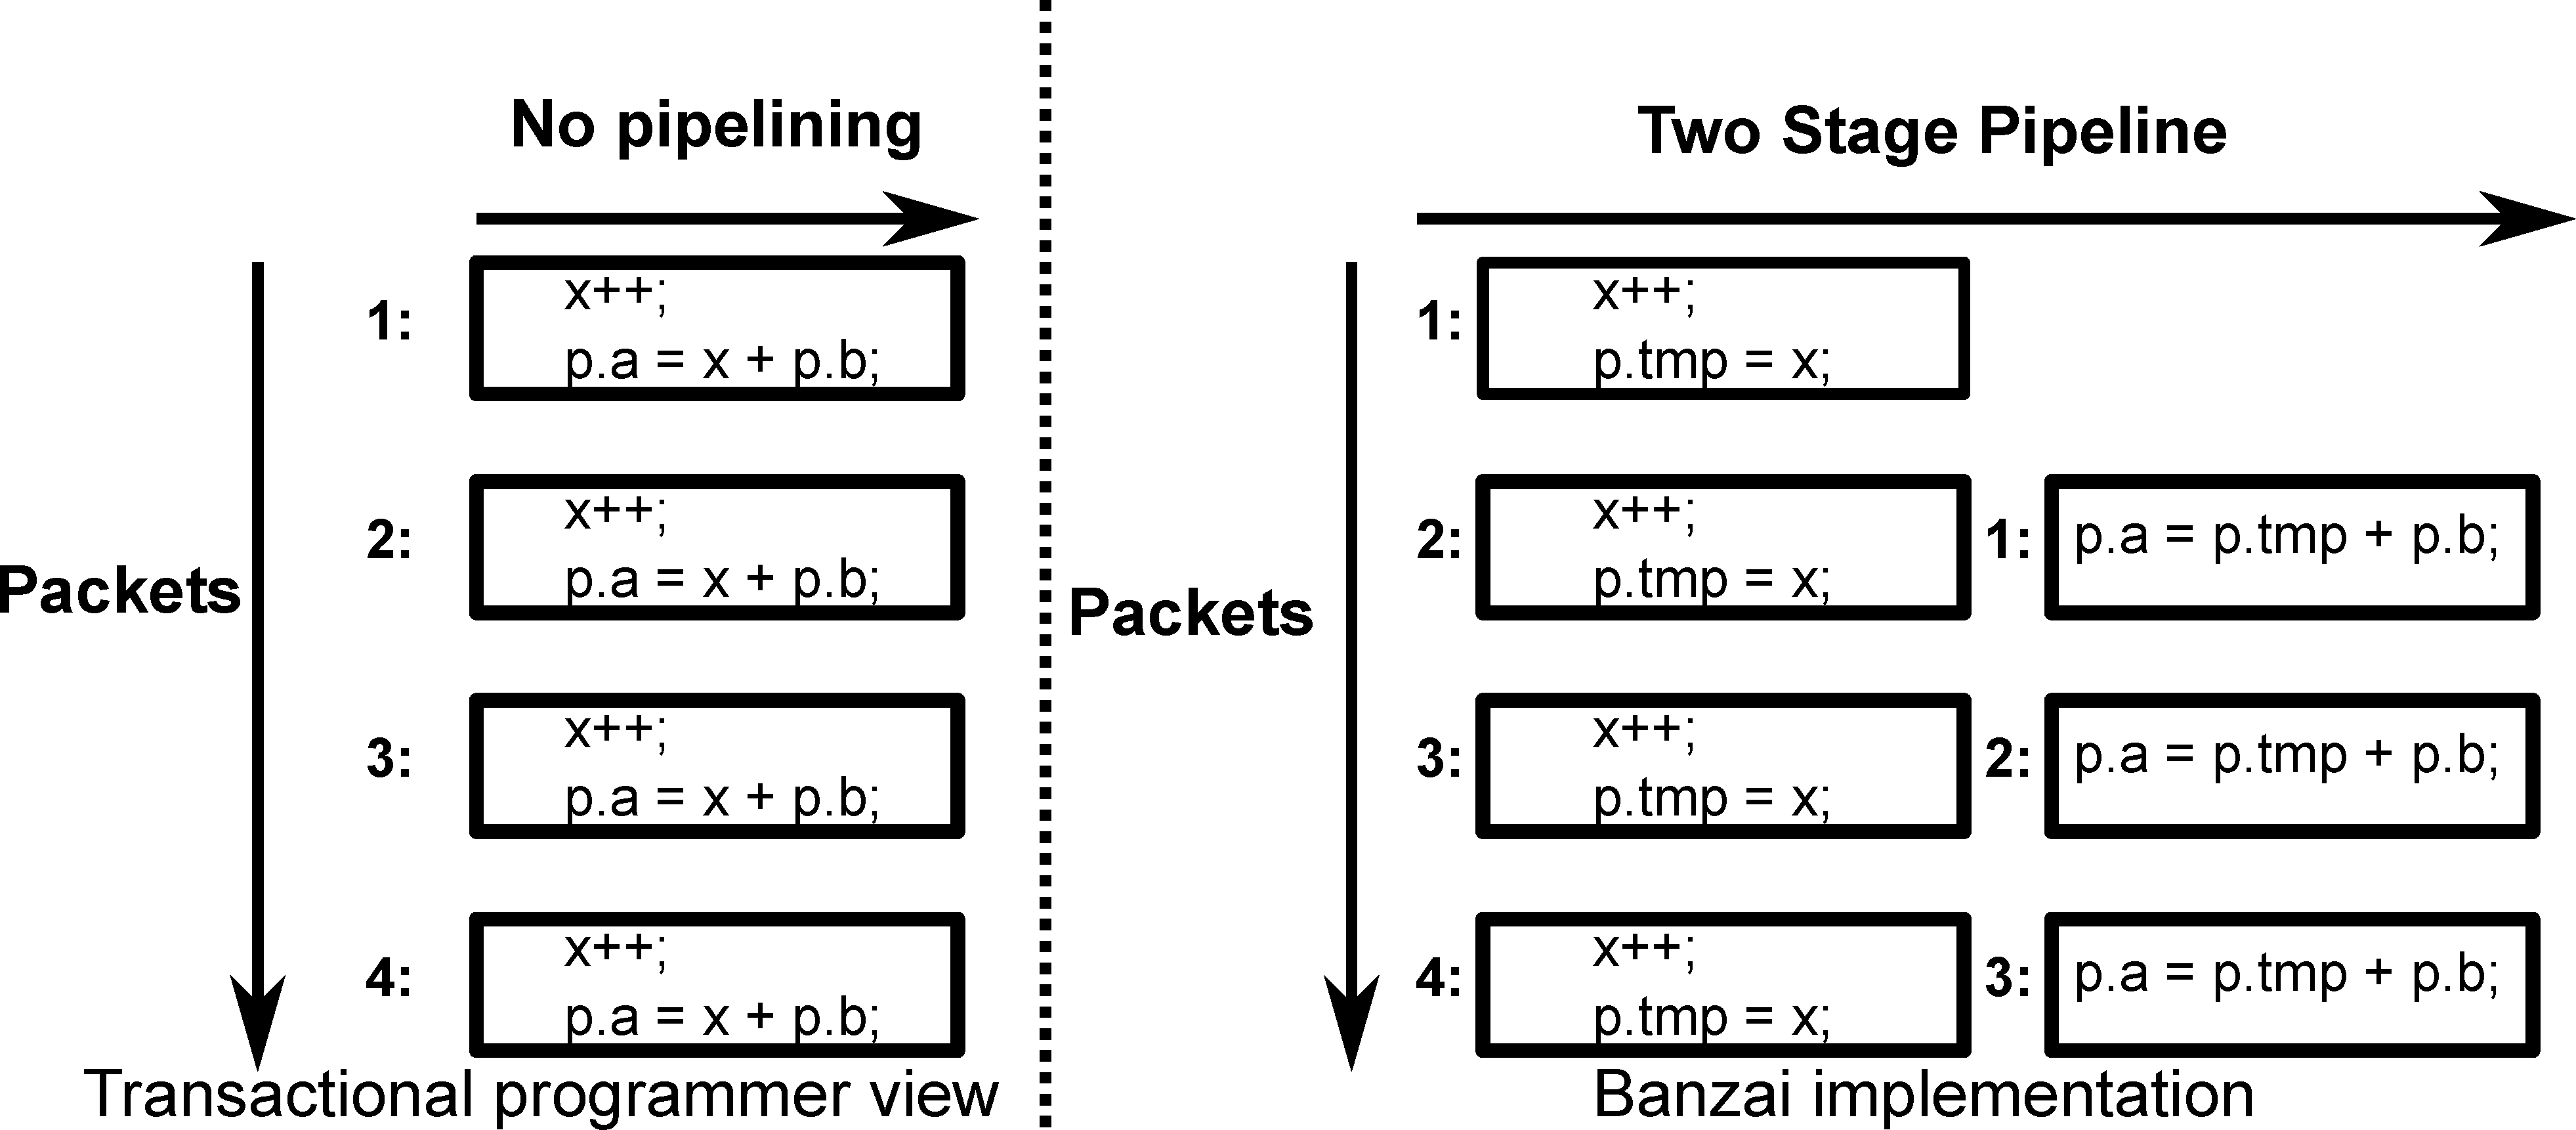
\includegraphics[width=\columnwidth]{spec_vs_impl.pdf}
%  \caption{A packet transaction and its implementation}
%  \label{fig:trans}
%\end{figure}

Transactions are the strongest guarantee that a database system can provide in
that the effect of a transaction is either entirely visible or not with no
intermediate state being visible to the outside world.

We repurpose database transactions for data-plane programming by defining a
\textit{packet transaction}: a body of sequential code that executes from start
to finish on each packet and conceptually processes only one packet at a time.
For a programmer, the packet transaction represents what happens to every
packet without having to worry about other packets that are currently being
processed by the switch, how many pipeline stages it has, and how to
parallelize code. Conceptually, every packet is processed in isolation and to
completion using a sequential block of code before the next packet's processing
begins.

% TODO: Add a flowlet switching example as a running example here.
As an illustration of programming in \pktlanguage, we consider how a programmer
would express a data-plane load-balancing algorithm such as flowlet
switching~\cite{flowlet} using domino. Flowlet switching is a load balancing
that harnesses the natural burstiness of TCP traffic to load balance set of
packets (called flowlets) separated by a large enough interval in time, called
the flowlet threshold. This flowlet threshold is chosen to ensure that packets
from flowlets taking different paths do not arrive out of order at a TCP
receiver, thereby causing it to reorder packets and degrade throughput.

Flowlet switching is conceptually simple to write down and can be expressed
as the C code block shown in:
\begin{figure}
\begin{scriptsize}
\begin{lstlisting}
#define NUM_FLOWLETS      8000
#define FLOWLET_THRESHOLD 5

struct Packet {
  int src_port;
  int dst_port;
  int src_addr;
  int dst_addr;
  int protocol;
  int new_hop;
  int arrival_time;
  int next_hop;
  int flow_hash;
};

int last_time [NUM_FLOWLETS] = {0};
int saved_hop [NUM_FLOWLETS] = {0};

void flowlet(struct Packet pkt) {
  pkt.new_hop   = hash6(pkt.src_port, pkt.dst_port,
                        pkt.src_addr, pkt.dst_addr,
                        pkt.protocol, pkt.arrival_time);
  if (pkt.arrival_time - last_time[hash5(pkt.src_port, pkt.dst_port, pkt.src_addr, pkt.dst_addr, pkt.protocol) \% NUM_FLOWLETS] >
      FLOWLET_THRESHOLD) {
    saved_hop[hash5(pkt.src_port, pkt.dst_port, pkt.src_addr, pkt.dst_addr, pkt.protocol) \% NUM_FLOWLETS] = pkt.new_hop;
  }
  last_time[hash5(pkt.src_port, pkt.dst_port, pkt.src_addr, pkt.dst_addr, pkt.protocol) \% NUM_FLOWLETS] = pkt.arrival_time;
  pkt.next_hop = saved_hop[hash5(pkt.src_port, pkt.dst_port, pkt.src_addr, pkt.dst_addr, pkt.protocol) \% NUM_FLOWLETS];
}
\end{lstlisting}
\end{scriptsize}
\label{fig:flowlet}
\caption{Flowlet switching in \pktlanguage}
\end{figure}

% TODO: Do we mention programmable parsers anywhere?
This packet transaction demonstrates the core language constructs in
\pktlanguage. All packet processing happens in the context of a packet
transaction, a C function that takes a packet structure as an argument.  In the
example above, this is the function \texttt{flowlet}. The function body of a
packet transaction can reference only two types of variables. Packet variables
are represented as structure members and persist only over the duration of a
packet, e.g. \texttt{pkt.next\_hop}). State variables are represented as global
variables and persist across packets, e.g. \texttt{last\_time}.

The function body may also call out to opaque functions such as hash5 and hash6
that represented hardware units provided by the abstract machine. The compiler
knows the function signatures for these units and uses these to infer
read-write dependencies between function arguments and the result, but doesn't
know anything about the function's implementation. Finally, the function body
is written in a heavily constrained subset of C that excludes iterative
constructs, break, goto, and continue statements, pointers, heaps.

% Anirudh->Alvin: Maybe move grammar into appendix?

% Anirudh->Alvin: I think we might want to get rid of a language section and
% just describe the language as part of this example itself?
%%Additionally,
%%\pktlanguage currently only handles scalar packet variables
%%Permits arrays with the same read and write addresses.

%The global arrays \texttt{last\_time} and \texttt{saved\_hop}
%represent the last time a packet was received from a given 5-tuple and the
%saved value of the next hop for that 5-tuple.\footnote{Hash function collisions
%  can occur, leading to two flows sharing last\_time and saved\_hop values. As
%we explain later in \S\ref{s:banzai}, this is unavoidable given the constraints
%on modern switch architectures.}. The next\_hop packet field specifies the next
%hop chosen for the packet, which can either be the saved value of next hop or a
%newly computed value.

When compiled to the \absmachine abstract machine, the \pktlanguage compiler
converts the above code into the pipelined form shown in
Figure~\ref{fig:pipeline}. Today, programmable switch chips are programmed by
manually specifying pipeline configurations using a language like P4 or an API
such as Cavium's XPliant SDK. Programming in \pktlanguage lets a compiler
automate this process: the user doesn't worry about hardware details such as
pipeline stages and concurrency within each stage.

%TODO: Insert a diagram of the pipeline here.
